%* 
%* ------------------------------------------------------------------
%* FCFReference.tex - FCF V2 reference
%* Created by Robert Heller on Sat Apr 21 13:30:23 2007
%* ------------------------------------------------------------------
%* Modification History: $Log$
%* Modification History: Revision 1.1  2007/05/06 12:49:39  heller
%* Modification History: Lock down  for 2.1.8 release candidate 1
%* Modification History:
%* Modification History: Revision 1.1  2002/07/28 14:03:50  heller
%* Modification History: Add it copyright notice headers
%* Modification History:
%* ------------------------------------------------------------------
%* Contents:
%* ------------------------------------------------------------------
%*  
%*     Model RR System, Version 2
%*     Copyright (C) 1994,1995,2002-2005  Robert Heller D/B/A Deepwoods Software
%* 			51 Locke Hill Road
%* 			Wendell, MA 01379-9728
%* 
%*     This program is free software; you can redistribute it and/or modify
%*     it under the terms of the GNU General Public License as published by
%*     the Free Software Foundation; either version 2 of the License, or
%*     (at your option) any later version.
%* 
%*     This program is distributed in the hope that it will be useful,
%*     but WITHOUT ANY WARRANTY; without even the implied warranty of
%*     MERCHANTABILITY or FITNESS FOR A PARTICULAR PURPOSE.  See the
%*     GNU General Public License for more details.
%* 
%*     You should have received a copy of the GNU General Public License
%*     along with this program; if not, write to the Free Software
%*     Foundation, Inc., 675 Mass Ave, Cambridge, MA 02139, USA.
%* 
%*  
%* 

\chapter{Freight Car Forwarder (V2) Reference}
\label{chpt:fcf:Reference}
\typeout{$Id$}

The Freight Car Forwarder (V2) is a hybrid program, consisting of a
Tcl/Tk GUI on top of a C++ class library.  The GUI provides the user
interface to the algorithms and data structures contained in the C++
class library.

\section{Command Line Usage}

The name of the system file to load can be specified on the command
line. See Section~\ref{sect:fcf:loadsystem} for more information.

\section{Layout of the Main GUI}

\begin{figure}[hbpt]
\begin{centering}
\includegraphics[width=5in]{FCFMain.png}
\caption{The main GUI screen of the Freight Car Forwarder (V2) Program}
\label{fig:fcf:FCFMain}
\end{centering}
\end{figure}
\begin{figure}[hbpt]
\begin{centering}
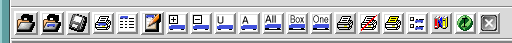
\includegraphics[width=5in]{FCFMainToolbar.png}
\caption{The Toolbar of the Freight Car Forwarder (V2) Program}
\label{fig:fcf:FCFMainToolbar}
\end{centering}
\end{figure}
\begin{figure}[hbpt]
\begin{centering}
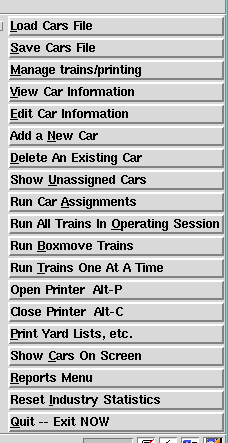
\includegraphics{FCFMainButtonMenu.png}
\caption{The Button Menu of the Freight Car Forwarder (V2) Program}
\label{fig:fcf:FCFMainButtonMenu}
\end{centering}
\end{figure}
\begin{figure}[hbpt]
\begin{centering}
\includegraphics{FCFMainIndicators.png}
\caption{The Indicators of the Freight Car Forwarder (V2) Program}
\label{fig:fcf:FCFMainIndicators}
\end{centering}
\end{figure}
The main GUI window\index{Freight Car Forwarder!main GUI}, show in
Figure~\ref{fig:fcf:FCFMain}, contains a menu bar, a toolbar
(Figure~\ref{fig:fcf:FCFMainToolbar}), a text display area, and a
button menu (Figure~\ref{fig:fcf:FCFMainButtonMenu}). There is also a 
work in progress message area, a  general status area, a progress
meter, and several indicators (Figure~\ref{fig:fcf:FCFMainIndicators}).
The main GUI also has three ``slide out'' frames, one for showing train
status when trains are run, one for viewing a car's information, and
one for editing a car's information. Each slide out has a corresponding
indicator. 

\section{Opening and loading a system file.}
\label{sect:fcf:loadsystem}
\index{Freight Car Forwarder!Loading a system file|(}

The \verb=File->Open...= menu button and the
\includegraphics{FCFLoadTool.png} toolbar button pop-up a file selection
dialog to select a system file to load. Once this file is successfully
loaded, the name of the file, the name of the system, the current
session and shift number, plus a count of  divisions, stations,
industries, cars, and trains is displayed in the main GUI's text area. 
Also all of the buttons are made active.  The name of the system file
can be specified on the command line and the named system file will be
loaded when the program starts.
\index{Freight Car Forwarder!Loading a system file|)}

\section{Loading and reloading the cars file.}

The \verb=Load Cars File= menu button and the

\includegraphics{FCFLoadCarsTool.png} toolbar button load (or reload)
the cars file.

\section{Saving the cars file.}

The \verb=Save Cars File= menu button and the 
\includegraphics{FCFSaveCarsTool.png} 
toolbar button save the cars and statistics files. This is something you
need to do after you have simulated a session, by running the car
assignment procedure and then run the trains in your session.  This
saves the state for the next time you run the Freight Car Forwarder.

\section{Managing trains and printing}
\begin{figure}[hbpt]
\begin{centering}
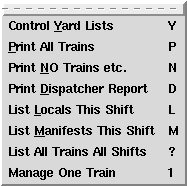
\includegraphics{FCFManageTrainsMenu.png}
\caption{Train/Printing Management Menu.}
\label{fig:fcf:FCFManageTrainsMenu}
\end{centering}
\end{figure}
The \verb=Manage trains/printing= menu button and the 

\includegraphics{FCFManageTrainsTool.png} toolbar button pop-up the
train/printing management menu.  This menu provides a set of functions
relating to what trains are printed and can also  print a dispatcher
report and generate lists of various sorts of trains.  The menu is shown
in  Figure~\ref{fig:fcf:FCFManageTrainsMenu}.

\subsection{Controling Yard Lists}

\begin{figure}[hbpt]
\begin{centering}
\includegraphics{FCFControlYardLDialog.png}
\caption{Control Yard Lists Dialog}
\label{fig:fcf:controlyardldialog}
\end{centering}
\end{figure}
The \verb=Control Yard Lists= menu item (y key) pops up a dialog, shown
in Figure~\ref{fig:fcf:controlyardldialog}, to control whether to print
0, 1, or 2 alphabetical lists and whether to print 0, 1, or 2 train
lists.

\subsection{Enabling printing for all trains}

The \verb=Print All Trains= menu item (p key) turns on printing for all
trains. 

\subsection{Disabling printing for all trains}

The \verb=Print No Trains= menu item (n key) turns off printing for all
trains.

\subsection{Printing a dispatcher report}

The \verb=Print Dispatcher Report= menu item (d key) enables the
printing of a dispatcher report.

\subsection{Listing local trains for this shift}

The \verb=List Locals This Shift= menu item (l key) lists all locals for
this shift.

\subsection{Listing manifests for this shift}

The \verb=List Manifests This Shift= menu item (m key) lists manifest
freights for this shift.

\subsection{Listing all trains for all shifts}

The \verb=List All Trains All Shifts= (? key) Lists all trains.

\subsection{Managing one train}

\begin{figure}[hbpt]
\begin{centering}
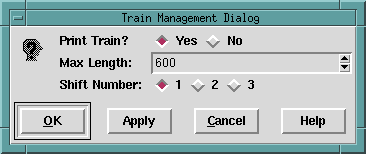
\includegraphics{FCFManage1TrainDialog.png}
\caption{Train Management Dialog}
\label{fig:fcf:manage1train}
\end{centering}
\end{figure}
The \verb=Manage One Train= menu item (1 key) pops up a dialog, shown
in Figure~\ref{fig:fcf:manage1train}, to enable or disable printing of
a single train, as well as setting the train's maximum length and
setting which shift the train will be run.  The train is selected with
the ``Select Train Dialog'', described in
Section~\ref{sect:fcf:selecttraindialog}.

\section{Viewing a car's information}

\begin{figure}[hbpt]
\begin{centering}
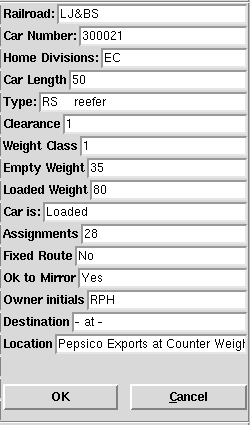
\includegraphics{FCFViewCarSlideout.png}
\caption{View Car Information Slideout}
\label{fig:fcf:viewcarslideout}
\end{centering}
\end{figure}
The \verb=View Car Information= menu button and the

\includegraphics{FCFViewCarTool.png} toolbar button display the
information about a single car.  The information is displayed on the
view car ``slide out'', shown in Figure~\ref{fig:fcf:viewcarslideout}.
The car is selected with the ``Search For Cars Dialog'', described in
Section~\ref{sect:fcf:searchcarsdialog}. 

\section{Editing a car's information}

\begin{figure}[hbpt]
\begin{centering}
\includegraphics{FCFEditCarSlideout.png}
\caption{Edit Car Information Slideout}
\label{fig:fcf:editcarslideout}
\end{centering}
\end{figure}
The \verb=Edit Car Information= menu button and the

\includegraphics{FCFEditCarTool.png} toolbar button display the
information about a single car and allow for editing this information. 
The information is displayed on the edit car ``slide out'', shown in
Figure~\ref{fig:fcf:editcarslideout}. The car is selected with the
``Search For Cars Dialog'', described in
Section~\ref{sect:fcf:searchcarsdialog}. 

\section{Adding a new car}

The \verb=Add a New Car= menu button and the

\includegraphics{FCFAddCarTool.png} toolbar button provide for adding a
new car.  The edit car ``slide out'', shown in
Figure~\ref{fig:fcf:editcarslideout} is displayed and the information
about the new car can be filled in and the car added.

\section{Deleting an existing car}

The \verb=Delete An Existing Car= menu button and the

\includegraphics{FCFDeleteCarTool.png} toolbar button provide for
deleting an existing car.  The car is selected with the ``Search For Cars
Dialog'', described in Section~\ref{sect:fcf:searchcarsdialog} and the
car's information is displayed in the view car ``slide out'', shown in
Figure~\ref{fig:fcf:viewcarslideout}. Actual removal can then be
confirmed.

\section{Showing cars without assignments}

The \verb=Show Unassigned Cars= menu button and the
\includegraphics{FCFShowUACarsTool.png} toolbar button display
unassigned cars in the text window.

\section{Running the car assignment procedure}

The \verb=Run Car Assignments= menu button and the

\includegraphics{FCFRunCarATool.png} toolbar button run the car
assignment procedure.  This procedure attempts to give as many
unassigned cars assignments, that is possible destinations. 
Considerations taken into account are the type of car, whether it is
loaded or not, industries with available trackage to accommodate the car,
and so on.  The list of cars is scanned twice and the progress of the
procedure is displayed in the text area.

\section{Running every train in the operating session}

\begin{figure}[hbpt]
\begin{centering}
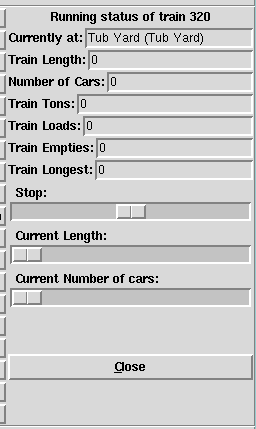
\includegraphics{FCFTrainStatusSlideout.png}
\caption{Train Status Slideout}
\label{fig:fcf:trainstatusslideout}
\end{centering}
\end{figure}
The \verb=Run All Trains in Operating Session= menu button and the
\includegraphics{FCFRunAllTrTool.png} toolbar button run all trains in
the operating session, except the end of session box moves.  Each
train's progress is shown in the ``Train Status Slideout'', shown in
Figure~\ref{fig:fcf:trainstatusslideout}.

\section{Running the boxmove trains}

The \verb=Run Boxmove Trains= menu button and the
\includegraphics{FCFRunBTrTool.png} toolbar button run all of the box
move trains in the operating session.  Each train's progress is shown
in the ``Train Status Slideout'', shown in
Figure~\ref{fig:fcf:trainstatusslideout}.

\section{Running a single train}

The \verb=Run Trains One At A Time= menu button and the

\includegraphics{FCFRun1TrTool.png} toolbar button run a single train,
selected with the ``Select Train Dialog'', described in
Section~\ref{sect:fcf:selecttraindialog}. The train's progress is shown
in the ``Train Status Slideout'', shown in
Figure~\ref{fig:fcf:trainstatusslideout}.


\section{Opening a Printer}

\begin{figure}[hbpt]
\begin{centering}
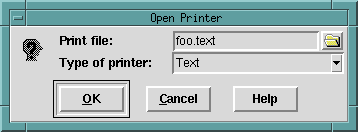
\includegraphics{FCFOpenPrinterDialog.png}
\caption{Open Printer Dialog}
\label{fig:fcf:openprinterdialog}
\end{centering}
\end{figure}
The \verb=Open Printer= menu button and the

\includegraphics{FCFOpenPrinterTool.png} toolbar button open the printer
output file, using the ``Open Printer Dialog'', shown in
Figure~\ref{fig:fcf:openprinterdialog}. The status of the printer
output, open or closed, is shown with the printer status indication,
\includegraphics{FCFPrinterInd.png}.

\section{Closing the printer}

The \verb=Close Printer= menu button and the
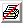
\includegraphics{FCFClosePrinterTool.png} toolbar button close the
printer.The status of the printer output, open or closed, is shown with
the printer status indication, \includegraphics{FCFPrinterInd.png}.

\section{Printing yard and switch lists}

The \verb=Print Yard Lists, etc.= menu button and the

\includegraphics{FCFPrintYardTool.png} toolbar button print the yard and
switch lists.

\section{Showing cars on the screen}

\begin{figure}[hbpt]
\begin{centering}
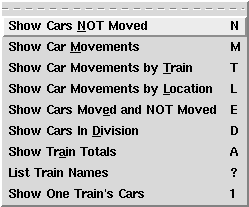
\includegraphics{FCFShowCarsMenu.png}
\caption{Show Cars Menu}
\label{fig:fcf:showcarsmenu}
\end{centering}
\end{figure}
The \verb=Show Cars On Screen= menu button and the
\includegraphics{FCFShowCarsTool.png} toolbar button pops up a menu,
shown in Figure~\ref{fig:fcf:showcarsmenu}, of classes of cars to show.

\section{Printing Reports}

\begin{figure}[hbpt]
\begin{centering}
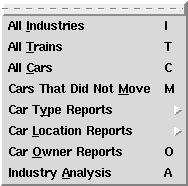
\includegraphics{FCFReportsMenu.png}
\caption{Reports Menu}
\label{fig:fcf:reportsmenu}
\end{centering}
\end{figure}
The \verb=Reports Menu= menu button and the
\includegraphics{FCFReportsTool.png} toolbar button pops up a menu,
shown in Figure~\ref{fig:fcf:reportsmenu}, of
possible reports.

\section{Reseting Industry Statistics}

The \verb=Reset Industry Statistics= menu button and the
\includegraphics{FCFResetStatsTool.png} toolbar button resets the
industry statistics.

\section{Quiting the application}

The \verb=Quit -- Exit NOW= menu button and the

\includegraphics{FCFCloseTool.png} toolbar button exit the program. A
confirmation dialog is popped up.


\section{General Dialogs}

\subsection{Control Yard Lists Dialog}
\subsection{Enter Owner Initials Dialog}

\subsection{Select A Train Dialog}
\label{sect:fcf:selecttraindialog}

\begin{figure}[hbpt]
\begin{centering}
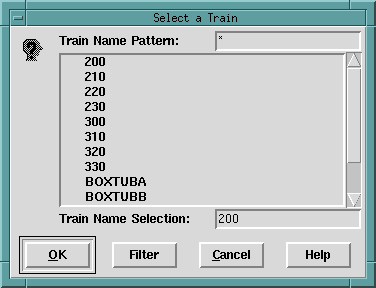
\includegraphics{FCFSelectATrainDialog.png}
\caption{Select A Train Dialog}
\label{fig:fcf:selecttraindialog}
\end{centering}
\end{figure}
The Select a Train Dialog is used to select a train (to manage, run, or
print). The \verb=Filter= button uses the Train Name Pattern to match
against train names to select a subset of trains to select from and can
contain these special sequences:  
\begin{itemize} 
\item \verb=*= Matches any sequence of zero or more characters in the
train name.
\item \verb=?= Matches any single character in the train name. 
\item \verb=[chars]= Matches any character in the set given by chars. 
If a sequence of the form \verb=x-y= appears in chars, then any
character between \verb=x= and  \verb=y=,  inclusive,  will match.
Characters are matched in a case insensitive way. 
\item \verb=\x= matches the single character \verb=x=. This provides a 
way of avoiding the special interpretation of the characters
\verb=*?[]\= in the pattern.
\end{itemize}

\subsection{Manage One Train Dialog}
\subsection{Open Printer Dialog}

\subsection{Search For Cars Dialog}
\label{sect:fcf:searchcarsdialog}

\begin{figure}[hbpt]
\begin{centering}
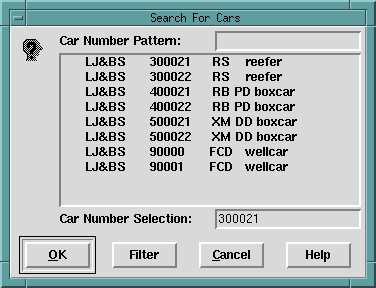
\includegraphics{FCFSelectACarDialog.png}
\caption{Search For Cars Dialog}
\label{fig:fcf:searchcarsdialog}
\end{centering}
\end{figure}
The Search For Cars Dialog is used to select a car (to view, edit, or
delete). The \verb=Filter= button selects a  subset of cars based on the
trailing car number digits.

\subsection{Select A Division Dialog}
\subsection{Select An Industry Dialog}
\subsection{Select A Station Dialog}
\subsection{Select Car Type}

\section{Data files}
\label{sect:fcf:Files}

The Freight Car Forwarder uses a collection of eight data files:

\begin{enumerate}
\item \verb=System File= This is the \textbf{master} file.  It contains the
(relative) paths to the remaining seven files, along with the name of
the railroad system, its divisions, and its stations.

\item \verb=Industry File= This file holds the description of the
industries, both on-line, which are actually modeled on the layout and
off- line, which are imaginary industries not actually on the layout,
but might be modeled as implied by staging yards or by interchange with
other layouts or imaginary off-line railroads.

\item \verb=Trains File= This file holds the description of the trains used
to actually move the cars about the layout.

\item \verb=Orders File= This file contains standing train orders and is
only used to add additional information to the printouts given to trail
operators.

\item \verb=Owners File= This file contains a mapping between owner initials
and owner names.  Used with various generated reports.

\item \verb=Car Types File= This file contains a mapping between car type
codes and full names and descriptions of car types.

\item \verb=Cars File= This is the file containing information about all of
the rolling stock on or off the layout.

\item \verb=Statistics File= This is the statistics file.  It is generated
by the program and contains statistical information about car and
industry utilization.
\end{enumerate}


\subsection{Data File Formats}
\label{sect:fcf:File Formats}

Some general notes:

A comment it indicated by an apostrophe.  All characters from the
apostrophe to the end of the line are discarded when read.  The files
generally contain lines of comma separated fields, a format
designed for BASIC read statements--the original program that this
program is based on was written in a version of BASIC and uses the same
file format.

\subsubsection{System File}

The first line of the system file is the name of the railroad system. 
This line is used in various banners and report headings.

The second line should be a blank line.

Then come the names of the remaining seven data files, one per line, in
this order: \verb=Industry File=, \verb=Trains File=, \verb=Orders File=, 
\verb=Owners File=, \verb=Car Types File=, \verb=Cars File=, and finally 
\verb=Statistics File=. 

After the file names comes the division list.  This starts with a count
of the maximum number of divisions:

\begin{verbatim}
Divisions = Number
\end{verbatim}

where Number is a positive non zero integer.

This is followed by division specifications, which is a list of 5 values
separated by commas:

\begin{verbatim}
Number,Symbol,Home,Area,Name
\end{verbatim}

Where Number is the index of the division (between 1 and the max number
of divisions, inclusive), Symbol is an alphanumeric character (a-z, 0-9,
A-Z), Home is the number of the home yard for this division (must be a
yard specified in the \verb=Industry File=), area is an Area symbol, and
Name is the name of the division.

A line containing a -1 terminates the list of divisions.

Then comes the stations (cities), starting with a line defining the maximum
number of stations:

\begin{verbatim}
Stations = Number
\end{verbatim}

where Number is a positive non zero integer.

This is followed by station specifications, which is a list of 4 values
separated by commas:

\begin{verbatim}
Number,Name,Division,Comment
\end{verbatim}

Where Number is the index of the station (between 1 and the max number
of stations, inclusive), Name is the name of the city, Division is the
division index, and Comment is commentary about the station. 
City/Station number one is used for the workbench.

A line containing a -1 terminates the list of stations.

\subsubsection{Industry File}

The industry file contains industries and yards.  The file starts with a
line specifying the maximum number of industries:

\begin{verbatim}
Industries = Number
\end{verbatim}

where Number is a positive non zero integer.

Followed by a line for each industry or yard.  Industry number 0 is
used for the repair yard, which is for cars not in service.  Each
industry's line contains these fields:

\begin{verbatim}
ID,T,STA,NAME,TLEN,ALEN,P,R,H,MIR,C,W,DCL,MAX,LD,EM
\end{verbatim}

Where:

\begin{description}
\item[ID]    Numeric identifier.
\item[T]     Types are \textbf{Y}ard or \textbf{I}ndustry or \textbf{O}ffline.
\item[STA]   Station Identifier.
\item[NAME]  User friendly place name.
\item[TLEN]  Actual or virtual track length.
\item[ALEN]  Assignable length.
\item[P]     Priority for car assignments. If \textbf{YARD} or \textbf{STAGE}, 
	\textbf{P} is $n$, the number of yard lists to print of type \verb=A=, 
	\verb=P=, or \verb=D=.
\item[R]     Reloads cars \textbf{Y}es or \textbf{N}o.
\item[H]     Hazard class for outbound cargo.
\item[MIR]   Mirror industry or 0 if none.
\item[C]     Maximum clearance plate.
\item[W]     Maximum weight class.
\item[DCL]   Destination Control List of divisions. If \textbf{YARD} or 
\textbf{STAGE}, DCL can contain:
  \begin{description}
  \item[A]     Alphabetical listing of cars in yard is permitted.
  \item[P]     Pickup listing of cars in yard is permitted.
  \item[D]     Dropoff listing of cars in yard is permitted.
  \end{description}
\item[MAX]   Maximum allowed car length.
\item[LD]    Loaded car types accepted.
\item[EM]    Empty car types accepted.
\end{description}

The industry listing is terminated by a line containing a -1.

\subsubsection{Trains File}

The trains file contains the trains used to move the cars.  The file
starts with a line specifying the maximum number of trains:

\begin{verbatim}
Trains = Number
\end{verbatim}

where Number is a positive non zero integer.

Followed by a record for each train (a newline is acceptable alternative
to a comma):

{\footnotesize
\begin{verbatim}
Number,Type,Shift,Done,Name,Maxcars, Divisions, Stops
	filler,Onduty,Print,Maxclear, Maxweight, Types,  Maxlen, 
	Description
\end{verbatim}
}

Where Number is the train number, Type is \textbf{M}anifest;
\textbf{B}oxmove; \textbf{W}ayfreight; or \textbf{P}assenger, Shift is
1; 2; or 3, Done is \textbf{Y}es or \textbf{N}o, Name is the train
name, Maxcars is the maximum number of cars, Divisions is a set of
division symbols or a wildcard (\verb=*=),Stops is a space separated
list of stations (Boxmove and Wayfrieghts) or industries (Manifests),
filler is an unused slot (use 0), Onduty is the time on duty (the
train's departure time) in the format HHMM, Print is \textbf{P}rint or
\textbf{N}oprint, Maxclear is the maximum clearance number, Maxweight
is the maximum weight number, Types is a set of car types this train
can carry, Maxlen is the maximum train length in feet, and Description
is a textual description of the train.

The train listing is terminated by a line containing a -1.

\subsubsection{Orders File}

This file contains lines with pairs:

\begin{verbatim}
Name,Order
\end{verbatim}

where Name is the name of a train and Order is a quoted string
containing the order.

\subsubsection{Owners File}

This file starts with a count of owners and then lines with with
triples:

\begin{verbatim}
Initials,Name,Comment
\end{verbatim}

where Initials are the three letter initials of an owner, Name is the
full name of the owner, and Comment is some descriptive text.

\subsubsection{Car Types File}

This is a file with exactly 91 records.  Each record contains:

\begin{verbatim}
Car Type Code,Car Type Group,Description,pad,Comment
\end{verbatim}

where Car Type Code is one of 91 printable characters, Car Type Group
is a single character, Description is a 16 character brief description,
pad is 0, and Comment is some descriptive text.

After the car types is the Car type groupings, which map groups of car
types into groups using the second single character, with lines
containing these fields:

\begin{verbatim}
Car Type Group,Description,Comment
\end{verbatim}

where Car Type Group is a single character, Description is a 16
character brief description, and Comment is some descriptive text.

\subsubsection{Cars File}

The cars file starts with three numbers, one per line:

\begin{verbatim}
Total shifts
Current shift
Max car count
\end{verbatim}

The first number is the total number of shifts, the second is the
current shift number (1, 2, or 3), and the third number is the maximum
number of cars in the file.

The remainder of the file is car records. This file must be kept in
[alphabetical order]! Each record contains:

{\footnotesize
\begin{verbatim}
Type,Marks,Number,Home,CarLen,ClearPlate,CarWeight,EmptyWt,
	LoadLimit,Loaded,Mirror?,Fixed?,Owner,Done,Last,Moves,Loc,
	Dest,NTrips,NAssigns
\end{verbatim}
}
Where Type is from car types file, Marks is the railroad reporting
marks (9 characters max), Number is the car number (8 characters max),
Home is car home division (from system file), CarLen is extreme car
length, ClearPlate is the clearance plate (from plate file), CarWeight
is car weight class (from weight file), EmptyWt is light weight in
tons, LoadLimit is load limit in tons, Loaded is \textbf{L}loaded or
\textbf{E}mpty, Mirror? is ok to mirror \textbf{Y}es or \textbf{N}o,
Fixed? is fixed route \textbf{Y}es or \textbf{N}o, Owner is car owner's
3 character initials (from owners file), Done is car is done moving for
this session \textbf{Y}es or \textbf{N}o, Last is last train to handle
the car from trains file,Moves is actual movements this session,Loc is
car's present location from industry file, Dest car's destination from
industry file, NTrips is number of car trips, and NAssigns is number of
car assignments.

\subsubsection{Statistics File}

The statistics is a file generated as an output and should not be hand
edited.  This file has two formats, V1 and V2.  V1 is the original
format used by the original BASIC program.  V2 is an improved version
that avoids getting the fields jammed together due to numerical overflow
(result numbers too large for the field sizes).

The first line of either format contains the statistics period number. 
If in the new format (V2), this number is followed by a comma.

The rest of file file contains lines of four numbers, either space
separated (V1) or comma separated (V2): industry index, car count, car
length, and statistics length.

\subsubsection{Other data files}

There are some additional data files, which are not actually loaded into
the system.  These are the plate, weight, and hazard files.  These are
just informational files that are used to map clearance plate, weight
class, and hazard levels of cars.


